\chapter{Implementación}

En este capítulo se explicará las implementaciones realizadas para poder llevar a cabo el proyecto, tanto como para conseguir la comunicación con el sensor utilizado, los cambios realizados en Aaaida para poder visualizar las mediciones del sensor y por último el despliegue de todo en la Raspberry Pi. 

\section{Comunicación con el sensor}

Para la realización del proyecto es necesario un sensor el cual se pueda comunicar y enviar los datos por bluetooth. En la empresa se dispone de una serie de sensores médicos de los cuales se utilizará un monitor de ritmo cardiaco, Zephyr BioHarness 3. 

\begin{figure}[htb]
\begin{center}
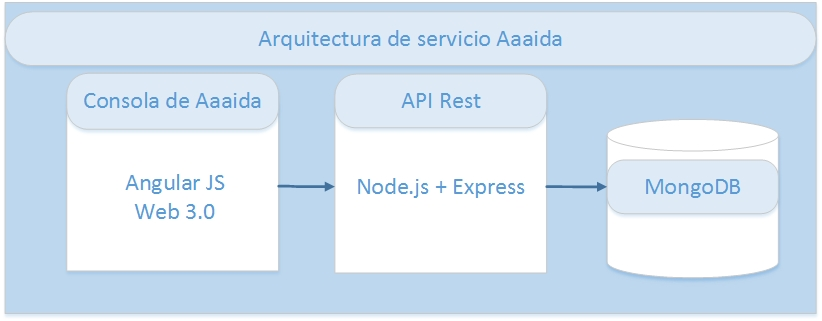
\includegraphics[width=1\textwidth]{./setup/arquitectura}
\caption{Sesor Zephyr BioHarness 3}
%\label{a:arquitectura}
\end{center}
\end{figure}

El fabricante te ofrece gran cantidad de documentación y una aplicación de prueba para los desarrolladores que quieran realizar productos y utilicen sus sensores. Pero todo está orientado a aplicaciones Android, las cuales son las más populares para este tipo de sensores. 

Por lo cual después de buscar y ponerse en contacto con la empresa no hay ningún tipo protocolo para establecer contacto y recibir los datos en JavaScript. Por lo tanto, se decidió realizar uno utilizando toda la documentación y ejemplos para otros lenguajes. 

Para la realización del código de comunicación fueron necesarios 2 módulos de Node.js uno que nos calcula el CRC y otro que establece una conexión bluetooth.

módulos utilizados:

\begin{itemize}
\item crc
\item bluetooth-serial-port 
\end{itemize}
\pagebreak

\subsection{Protocolo}

El código realizado para poder establecer la comunicaciones fue el siguiente.
 
Se cargan los módulos externos y se declaran las variables, la dirección MAC del sensor se pone a clavo para evitar interferencias con otros dispositivos bluetooth.

\begin{verbatim}
var crc = require('crc');
var btSerial = new (require('bluetooth-serial-port')).BluetoothSerialPort();

ADDRESS = "E0:D7:BA:A7:F1:5D";
var results = [];
var is_stopping = false;
\end{verbatim}

Función \texttt{connect}, como su nombre indica nos conectara con el sensor y empezará a recibir datos. 

\begin{verbatim}
function connect(callback) {
   var socket = btSerial.on('found', function (address) {
       if (address == ADDRESS) {
           btSerial.findSerialPortChannel(address, function (channel) {
               btSerial.connect(address, channel, function () {
                   console.log('connected to ' + address);
                   btSerial.on('data', function (buffer) {
                       decode(buffer);
                   });
                   listener(socket, function (res) {
                       callback(res);
                   });
               }, function () {
                   console.log('cannot connect');
               });
           }, function () {
               console.log('found nothing');
           });
       }
   });
   btSerial.inquire();
}
\end{verbatim}

La función \texttt{decode} nos permite decodificar de una manera muy simplificada los bytes que recibimos. Le pasamos el 2 byte y según su valor podremos saber qué tipo de mensaje nos está enviado el sensor. 

\begin{verbatim}
function decode(data) {
   switch (data[1]) {
       case 35:
           console.log("Received LifeSign message");
           break;
           \end{verbatim}
           \pagebreak
           \begin{verbatim}
       case 44:
           console.log("Received Event message");
           results.push(data[8]);
           break;
       case 43:
           console.log("Received Summary Data Packet");
           break;
       case 37:
           console.log("Received Accelerometer Data Packet");
           break;
       case 36:
           console.log("Received R to R Data Packet");
           break;
       case 33:
           console.log("Received Breathing Data Packet");
           break;
       default:
           console.log("Packet type: " + data[1]);
           console.log("Received Not recognised message");
           break;
   }
}
\end{verbatim}

Una vez conectados al sensor se debe enviar mensajes a este para que mantenga la conexión y no se desconecte (\texttt{lifeSings}). Como la finalidad es realizar una medida la comunicación se realizará durante 20 seg, una vez pasados estos 20 seg se cerrara la conexion. 

\begin{verbatim}
function listener(socket, callback) {
   socket.on('data', function (buffer) {
       decode(buffer);
       lifeSing = create_message_frame('100011', 0);
       socket.write(new Buffer(lifeSing), function (err, bytesWritten) {
           if (err) console.log(err);
       });
   });
   setTimeout(function () {
       stop(socket, function (res) {
           callback(res);
       });
   }, 20000);
}
\end{verbatim}

La creación de los mensajes \texttt{lifeSings} se realizan de la siguiente manera: Son la concatenación de un byte de sincronismo, el mensaje, el dlc que será la longitud del payload, el crc calculado mediante el payload y por ultimo otro byte de cierre. Todo paquete se pasará a hexadecimal y se procederá a enviarlo.
 \pagebreak
\begin{verbatim}
function create_message_frame(message_id, payload) {
   dlc = payload.toString().length;
   if (0 <= dlc <= 128) {
       crc_byte = crc.crc32(payload);
       message_bytes = '00000010'+ message_id + dlc + payload + crc_byte 
       + '00000011';
       message_fame = Bin2Hex(message_bytes);
       return message_fame
   }
}
\end{verbatim}

Por último la función de \texttt{stop} y la función de \texttt{avg}, la función de \texttt{stop} cerrará la conexión y la función de \texttt{avg} calcula la media de todas las medidas tomadas durante los 20 seg y devolverá la media. 

\begin{verbatim}
function stop(socket, callback) {
   is_stopping = true;
   socket.close();
   avg(function (res) {
       callback(res);
   });

}

function avg(callback) {
   var sum = 0;
   if (is_stopping == true) {
       for (var i = 0; i < results.length; i++) {
           sum = sum + results[i];
       }
       var media = sum / results.length;
       callback(media);
   }
}
\end{verbatim}

Con esto podremos establecer una conexión con el sensor y poder recibir la media del pulso cardiaco durante 20 seg. Hay que tener en cuenta la simplicidad del protocolo ya que solo capturamos una de las funciones (ritmo cardíaco) que nos proporciona el sensor Zephyr ya que si quisiéramos poder obtener todos los datos la complejidad sería mucho mayor y para desarrollarlo en JavaScript se necesitaría mucha más información sobre cómo se envían las tramas y que contiene cada una de ellas. 